\chapter{Réalisation}
\begin{onehalfspace}

\initial{C}e chapitre est consacré à la description de la phase de la réalisation. La démarche globale de deux solutions sera décrite, puis les avantages de l'une par rapport à l'autre seront illustrés. Enfin, La sécurisation et l'installation d'un système de supervision scalable cloturera le chapitre.

\newpage

\section{A base d'un Cluster}

\subsection{Installation du Cluster}

Nous allons mettre en place l'architecture décrite dans la figure \ref{fig:architecture}). 


\begin{itemize}
	\item \textbf{Réseau privé} : Les serveurs du Cluster communiquent entre eux avec des adresses \acrshort{ip} privées. Cette solution est contraignante. En effet, les serveurs doivent être installés dans la même zone. De plus les fournisseurs chargent des coûts supplémentaires pour l'installation d'une interface réseau privée. En contrepartie, on gagne en termes de sécurité;
	\item \textbf{Réseau public} : Les serveurs du Cluster peuvent se communiquer mutuellement via une interface réseau public et donc une adresse \acrshort{ip} public. De ce fait, beaucoup d'avantages se dégagent. D'une part, les serveurs peuvent être distribués dans le monde entier et ainsi garantir une disponibilité maximale. D'autre part, une migration à chaud de toute la plate-forme peut être faite. Cette migration est silencieuse et transparente pour tous les clients.
\end{itemize}

\subsection{Installation des proxy}
\index{Gogeta}

\textbf{Gogeta} est un proxy dynamique dont la configuration est basée sur la base de donnée Etcd. En effet, Gogeta écoute en permanence Etcd pour assurer une reconfiguration dynamique en temps réel des routes sans redémarrage.

Quand l'ordonnanceur Fleet crée un service en mode haute disponibilité, Il stocke les donnée (\acrshort{ip} et port) dans Etcd sous forme de clé-valeur. Les proxy Gogeta, étant en écoute en permanence d'Etcd , se reconfigure pour prendre en considération le nouveau service. Ainsi, si une requête arrive sur l'un des proxy Gogeta, il la transmet vers une des instances avec la stratégie \emph{Round-robin} après avoir fait des bilans de santé.

\begin{lstlisting}[language=bash,caption=Contenu de la base de donnée Etcd]
	/domains/odoo.sayoo.org/value 	= odoo
	/services/odoo/1/location		= {"host":"10.240.210.86", "port": 42654}
	/services/odoo/2/location		= {"host":"10.240.228.23", "port": 42669}
\end{lstlisting}


La solution à base d'un cluster CoreOS motorisé par des équilibreurs de charges élastique est très puissante, mais son utilisation demeure très bas niveau. Le fait d'interagir directement avec le cluster nécessite des administrateurs systèmes très compétents. C'est la raison pour laquelle nous allons essayer d'adopter une solution à base d'une \acrshort{paas}.


\section{A base d'une \acrshort{paas}}
\index{Deis}
\subsection{Plate-forme Deis}

\subsubsection*{Deis}

\begin{wrapfigure}{l}{3cm}
\centering

\includegraphics[scale=0.4]{chapitre5/assets/deis}
\end{wrapfigure}
\noindent \emph{Deis} est une Plate-forme en tant que service, \acrshort{paas}, open-source qui facilite la gestion et le déploiement des applications sur des serveurs. Deis se base sur Docker et CoreOS pour fournir une \acrshort{paas} très légère inspirée par la fameuse plate-forme Heroku.


\subsubsection*{Applications supportées}

Deis peut déployer n'importe quelle application ou service qui peut fonctionner à l'intérieur d'un conteneur Docker. Pour que l'application soit évolutive horizontalement, elles doivent suivre la méthodologie de 12-facteur de Heroku (Voir Annexe \ref{annexe:12factors}, page \pageref{annexe:12factors}).

\subsubsection*{Plates-formes supportées}
Deis peut être déployée sur un n'importe quelle système qui supporte CoreOS : poste de travail, ainsi que la plupart des Clouds publics, privés et les centres de données.


\subsubsection*{Pourquoi Deis?}

\begin{itemize}
	\item Langage-agnostique: Deis déploie des services écrites dans n'importe quels langages avec une simple commande "git push";
	\item Extensibilité: Deis est extensible, les outils de supervisions et de la gestions des messages logs peuvent être intégrés facilement;
	\item Scalabilité: Une application est montée en charge avec une seule commande. Par ailleurs, La capacité de la plate-forme Deis peut être montée en charge en ajoutant simplement des hôtes au cluster;
	\item 100\% Open Source: Deis est un logiciel libre, open-source publié sous la licence Apache 2.0.
\end{itemize}


\subsection{Architecture}

l'architecture de Deis présentée dans la figure \ref{fig:deis-architecture} a tellement de points de commun avec celle que nous avons proposé. Néanmoins, elle cache beaucoup de détails, notamment à l'intérieur du contrôleur où beaucoup de magie se fait. Par ailleurs, Deis intègre ses propres routeurs (équilibreurs de charges) et un registre privé des images Docker. Les services de support, la supervision, la gestion des messages logs et l'équilibreur de charge ne sont pas intégrés par la plate-forme Deis.

Un développeur, voulant déployer une application, va pousser son code vers le contrôleur. Ce dernier construit l'image et la stocke dans le registre des images. Ensuite, le contrôleur passe le relais à l'ordonnanceur qui se débrouille pour lancer le service à l'intérieur d'un conteneur. Le conteneur est crée à base de l'image Docker.



\begin{figure}[H]
\centering
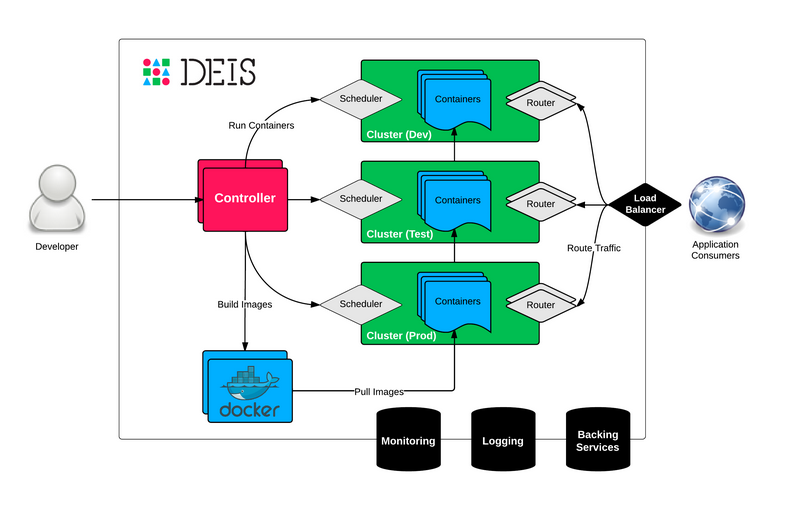
\includegraphics [scale=0.6]{chapitre5/assets/deis-architecture}
\caption{Architecture de la PaaS Deis}
\label{fig:deis-architecture}
\end{figure}


\subsection{Installation}


Deis nécessite un Cluster de CoreOS pour s'installer dessus. Nous aurions pu installer Deis au-dessus du Cluster que nous avons déjà réalisé, mais Deis nécessite des ressources (au moins 4GB de RAM) que la version d'essai de \acrshort{aws} n'offre pas. Nous avons opté pour \acrshort{gce}.

L'installation de Deis sur \acrshort{gce} est détaillé dans la documentation \cite{deis-gce}. Les grandes étapes d'installation:
\begin{itemize}
	\item Lancer des serveurs CoreOS avec le fichier d'initialisation de Deis fournit par la documentation;
	\item Faire pointer l'équilibreur de charge de Google vers nos serveurs. Cette équilibreur de charge est élastique et donc reconnaît dynamiquement des nouveaux serveurs;
	\item Configurer le \acrshort{dns} pour faire pointer le nom de domaine et tous les sous-domaines vers l'équilibreur de charge de Google (Figure \ref{fig:dns}).
\end{itemize}

\begin{figure}[H]
\centering
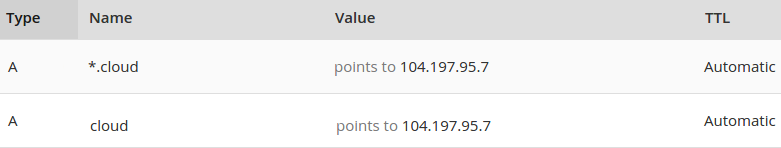
\includegraphics [scale=0.55]{chapitre5/assets/dns}
\caption{Configuration du DNS}
\label{fig:dns}
\end{figure}


\subsection{Avantages du \acrshort{paas} par rapport au Cluster}

\subsubsection*{Déploiement avec une seule commande}

	Quand le développeur a terminé le développement ou la personnalisation une application, il peut la déployer rapidement.

	\begin{lstlisting}[language=bash,caption=Déploiement avec Deis]
		$ git push deis master
	\end{lstlisting}

\subsubsection*{Montée en chargé avec une seule commande}

Après avoir lancé un service, l'exploitant, remarquant un pic de charge, va pouvoir ajouter d'autres instances du service. Les routeurs sont dynamiquement reconfigurés pour diffuser la charge à travers toutes les instances.

	\begin{lstlisting}[language=bash,caption=Montée en charge]
		$ deis scale cmd=3
	\end{lstlisting}

\subsubsection*{Déploiement avec zéro temps d'arrêt}

Durant le déploiement d'une nouvelle version d'un service, Deis garantit un zéro temps d'indisponibilité. En effet, les routeurs ne sont reconfigurés que lorsque le déploiement est terminé. Enfin, l'ancienne version est supprimée.


\subsubsection*{Des \acrshort{api} \acrshort{http}}

Deis offre des \acrshort{api}s REST pour un interfaçage facile et standard. Du coup, il est possible de développer dans le futur des interfaces web ou mobile qui cache les difficultés de la ligne de commande. D'ailleurs, une interface web est déja crée par la communauté pour la gestion du Cluster \cite{deis-ui}.





\subsection{Sécurité avec le protocole \acrshort{ssl}/\acrshort{tls}}

\subsubsection{\acrshort{ssl}/\acrshort{tls}}

\index{SSL}
\index{TLS}

\acrshort{ssl} est un protocole qui permet d'échanger des informations entre 2 ordinateurs de façon sûre. \acrshort{ssl} assure 3 choses:

\begin{itemize}
	\item \textbf{Confidentialité}: Il est impossible d'espionner les informations échangées;
	\item \textbf{Intégrité}: Il est impossible de truquer les informations échangées;
	\item \textbf{Authentification}: Il permet de s'assurer de l'identité du programme, de la personne ou de l'entreprise avec laquelle on communique.
\end{itemize}



Nous allons installer \acrshort{ssl} dans la plate-forme pour établir un lien crypté entre le navigateur et serveur (\acrshort{https}). Ce qui est intéressant, c'est que lorsque \acrshort{ssl} est activé pour le cluster, il le sera pour toute les services qui s'exécute sur le cluster.



\subsubsection{Installation}

L'installation de SSL dans la plate-forme se fait en 2 étapes:
\begin{itemize}
	\item Générer d'une clé privée et une certificat signée. Normalement, la certificat doit être signé par les PKI, des parties tierces aux-quelles l'on fait confiance, qui chargent une somme d'argent annuelle. Dans un environnement de test, on peut se contenter par une certificat que nous allons signer nous même;
	\item Attacher la clé privée et la certificat avec la plate-forme. En fait, elles doivent être installées dans l'équilibreur de charge. Il y a deux choix qui se portent à nous, soit les installer dans notre équilibreur de charge de \acrshort{gce} ou dans les proxy de Deis. Nous avons décidé de l'installer dans les équilibreurs de charge propres à Deis vu que c'est une solution portable et ne dépend pas de l'environnement où Deis est installé.
\end{itemize}

\begin{lstlisting}[language=bash,caption=Génération de la clé privée et la certificat]
	$ openssl genrsa -des3 -passout pass:x -out server.pass.key 2048
	$ openssl rsa -passin pass:x -in server.pass.key -out server.key
	$ openssl req -new -key server.key -out server.csr
	$ openssl x509 -req -days 365 -in server.csr -signkey server.key -out server.crt
\end{lstlisting}

\begin{lstlisting}[language=bash,caption=Activation du protocole SSL]
	$ deisctl config router set sslKey=server.key sslCert=server.crt
	$ deisctl config router set enforceHTTPS=true
\end{lstlisting}

\begin{figure}[H]
\centering
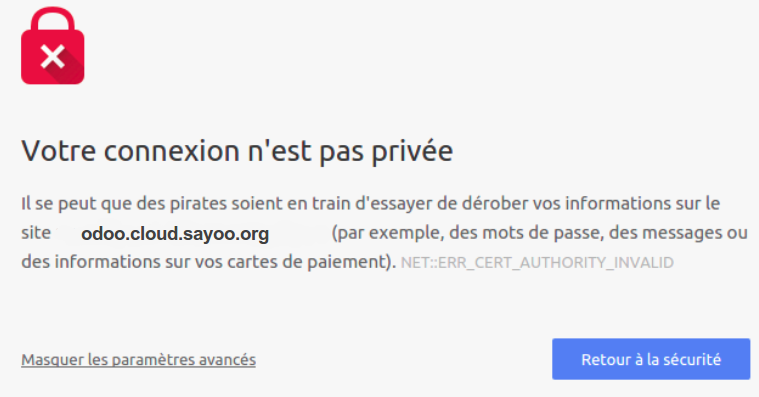
\includegraphics [scale=0.5]{chapitre5/assets/certificat}
\caption{Certificat non fiable}
\label{fig:certificat}
\end{figure}

Après avoir activé le protocole \acrshort{https}, le navigateur envoie un avertissement (Figure ~\ref{fig:certificat}, page~\pageref{fig:certificat}). En effet, nous avons signé la certificat nous-même au lieu de la déléguer à une partie tierce de confiance (\acrshort{pki}), ce qui devrait être fait en production. En dépit de cela, nous avons bel et bien sécurisé la communication (Figure ~\ref{fig:https}, page~\pageref{fig:https}).

\begin{figure}[H]
\centering
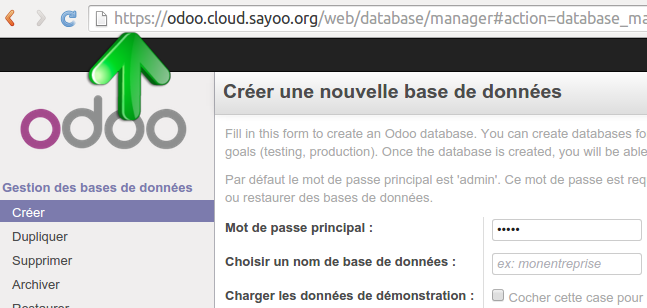
\includegraphics [scale=0.5]{chapitre5/assets/https}
\caption{Communication sécurisée avec le protocole \acrshort{https}}
\label{fig:https}
\end{figure}


\section{Supervision}

La \acrshort{paas} \emph{Deis} ne dispose pas d'un système de supervision intégré. Puisque les services déployés dans Deis fonctionnant entièrement à l'intérieur des conteneurs Docker, cela signifie que les outils de supervision des conteneurs Docker devraient fonctionner avec Deis. L'on va utiliser les plus matures d'entre eux.


\subsection{Outils de supervision utilisés}

	
\subsubsection*{cAdvisor}

\index{cAdvisor}

\begin{wrapfigure}{l}{3.5cm}
\centering

\includegraphics[scale=0.2]{chapitre5/assets/cadvisor}
\end{wrapfigure}
\noindent \emph{cAdvisor} (Container Advisor) fournit aux utilisateurs de conteneurs une vue de l'utilisation des ressources et des caractéristiques de performance de leurs conteneurs en cours d'exécution. C'est un démon, toujours en exécution, qui recueille, agrège, analyse, et exporte informations sur l'exécution des conteneurs. Plus précisément, pour chaque conteneur, il conserve l'historique de l'utilisation des ressources, les histogrammes des historiques complets d'utilisation des ressources et des statistiques du réseau. Ces données peuvent être exportées pour chaque conteneur ou pour toute la machine.

cAdvisor a un support natif pour les conteneurs Docker et devrait supporter à peu près tout autre solution de containérisation. Par ailleurs, cAdvisor fournit une interface utilisateur ainsi qu'une REST API.


\subsubsection*{Heapster}

Heapster est un projet open source de Google qui comble la limitation de cAdvisor qui supervise un seul serveur. Heapster recueille les données à travers les \acrshort{http} \acrshort{api} fournit par les cAdvisor installés sur les serveurs, puis les stocke dans la base de donnée InfluxDB. Ainsi, Heapster est considéré comme un superviseur au niveau du Cluster.

\subsubsection*{InfluxDB}

\begin{wrapfigure}{l}{3.5cm}
\centering

\includegraphics[scale=0.2]{chapitre5/assets/influxdb}
\end{wrapfigure}
\noindent Influxdb est une base de donnée distribuée destinée pour le stockage des métriques, des événements et des analyses de performances. Influxdb est simple à installer et à gérer, et rapide car il vise à répondre aux requête en temps-réel. En effet, chaque point de données est indexé et disponible pour des requêtes qui retournent des réponses dans < 100 ms. Enfin, il dispose d'une \acrshort{http} \acrshort{api} intégré qui va être sollicitée par l'interface utilisateur Grafana.

\subsubsection*{Grafana}

\begin{wrapfigure}{l}{3.5cm}
\centering

\includegraphics[scale=0.3]{chapitre5/assets/grafana}
\end{wrapfigure}
\noindent Grafana est l'un des meilleurs projets open source pour la visualisation des données de mesure. Il fournit un moyen puissant et élégant pour créer, partager et explorer les données et les tableaux de bord à partir des bases de données de métriques. Grafana assure un support riche pour les bases de données Graphite, InfluxDB et OpenTSDB. Grafana sera utilisé pour visualiser les mesures stockées dans InfluxDB.


\subsection{Démarche d'installation}

Cette solution de supervision s'installe au-dessus du Cluster de CoreOS et cohabite avec la plate-forme Deis. Comme c'est déjà mentionné, tous les services sous CoreOS sont installés en tant que conteneur. De même, cAdvisor, InfluxDB, Heapster et Grafana vont être installés dans des conteneurs.
Les fichiers d'installation se trouvent dans le guide officielle de Heapster \cite{heapster-coreos}

\begin{itemize}
	\item cAdvisor doit être installé sur tous les serveurs du cluster. Heureusement, l'ordonnanceur Fleet effectue cette opération de façon automatique et scalable. En effet, il suffit de mentionner \emph{Global=true} dans le fichier d'installation;
	\item InfluxDB, Heapster et Grafana doivent être installé dans le même serveur. L'on exprime cette contrainte par \emph{X-ConditionMachineOf=influxdb.service}. Ainsi, Fleet va s'en sortir pour faire coexister les trois services.
\end{itemize}

\begin{figure}[H]
\centering
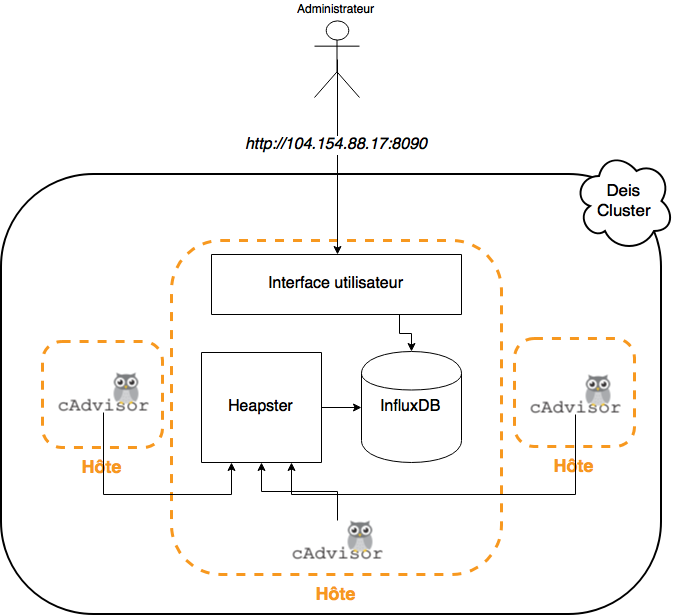
\includegraphics [scale=0.6]{chapitre5/assets/monitoring-cluster}
\caption{Architecture de la supervision}
\label{fig:}
\end{figure}

Le code suivant montre comment charger et installer cAdvisor dans le cluster. C'est la même procédure pour les autres services.

\begin{lstlisting}[language=bash,caption=Lancement du service cAdvisor]
	$ ssh core@104.154.75.6 
	$ fleetctl load cadvisor.service
	$ fleetctl start cadvisor.service
\end{lstlisting}


\subsection{Interfaces graphique}

Notre cluster se compose de trois serveurs. Les figures suivantes présentes la quantité totale de \acrshort{cpu} et de la mémoire consommée par le cluster ainsi que les quantités consommées par chaque serveur.

\begin{figure}[H]
\centering
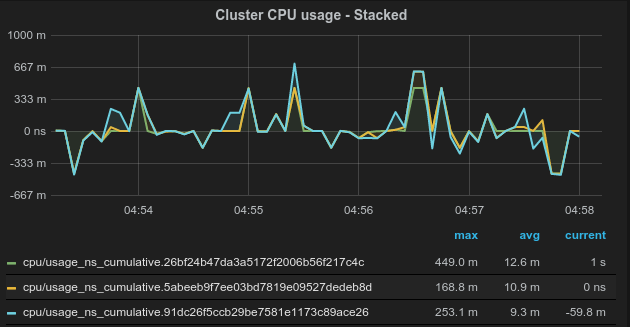
\includegraphics [scale=0.6]{chapitre5/assets/cluster-cpu}
\caption{Quantité de CPU consommées par le cluster}
\label{fig:}
\end{figure}

\begin{figure}[H]
\centering
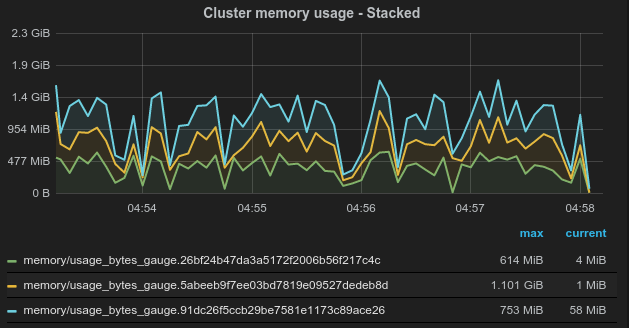
\includegraphics [scale=0.6]{chapitre5/assets/cluster-memory}
\caption{Quantité de mémoire consommées par le cluster}
\label{fig:}
\end{figure}


\subsection{Supervision et scalabilité}

La scalabilité était toujours parmi nos aspirations tout au long de ce projet. Le système de supervision réalisé est conçu pour fonctionner de façon indépendante, complètement automatisée et hautement scalable. Cela va être prouvé à travers ces deux scénarios:

\begin{itemize}
	\item Quand un nouveau service est lancé sur un des serveurs du cluster, cAdvisor se rendra compte de ce nouveau conteneur et va mettra à la disposition de Heapster les données qui va les stocker dans la base de données pour des consultations via l'interface graphique;
	\item Lors d'un pic de charge, on a intérêt à lancer les nouveaux conteneurs dans un nouveau serveur. On va tout d'abord lancer avec le fichier d'initialisation du cluster. Désormais, de façon automatique, le serveur appartient au cluster. Ainsi, les conteneurs lancés sur ce nouveau serveur sont supervisés automatiquement comme le décrit le scénario 1.
\end{itemize}

D'autre part, Grafana, l'interface utilisateur, sera disponible dans la machine dans laquelle \emph{Fleet} décide d'installer le trio Heapster, InfluxDB et Grafana. Cela signifie que Grafana peut changer de position dans le cluster à l'improviste et n'aura donc pas une adresse \acrshort{ip} fixe pour y accéder. Comme perspective, il serait préférable de mettre en place une sorte de proxy dont l'\acrshort{ip} est fixe par lequel on accède à Grafana partout où il soit.


\section*{Conclusion}

Nous avons décrit l'installation et l'utilisation d'une plate-forme en tant que service au-dessus d'un Cluster de CoreOS. La \acrshort{paas}, couplée avec son interface utilisateur et un système de supervision, devient plus complète et favorise le déploiement continue dans un monde containérisé.

\end{onehalfspace}
